\section{Introduction}
Proton exchange membrane fuel cells (PEMFCs), henceforth denoted as fuel cells, facilitate the direct conversion of chemical energy present in hydrogen into electrical energy.
These fuel cells are characterized by their high energy utilization rate, low operating temperature, and the production of water as the sole reaction byproduct.
Their versatility allows them to function not only as a small-scale distributed power supply but also as the energy source for high-power transportation systems, thus demonstrating their broad applicability \cite{sharafOverviewFuelCell2014} .
Nevertheless, the reliability, stability, and durability of the fuel cell stack, as the central component of the fuel cell power system, have emerged as critical factors influencing the extensive commercialization of fuel cell products.
During the operational phase of the fuel cell, it is imperative to maintain the internal proton exchange membrane (PEM) in an optimal state of hydration to ensure the proton conduction ability remains at its peak, thereby achieving efficient and stable output performance of the fuel cell. Hydration state failure is the most prevalent failure mode of fuel cells, accounting for approximately 52 of total failures, primarily manifested as drying and flooding. Short-term hydration state failure can induce fluctuations and reductions in the output performance of the fuel cell. If this condition persists, it may lead to irreversible attenuation.
\par
Under dry failure, the water content inside the stack is too low to keep an sufficiently hydrated state,
and the internal resistance increases and heat production increases since some region of the PEM are not fully hydrated.
Long-term dryness may even cause mechanical damage to the PEM, resulting in irreversible damage\cite{pattersonDamageCathodeCatalyst2006}.
Under flooding failure, the water content inside the stack is too high, and the liquid water gradually block the flow channel or reaction area,
preventing the reaction gas from reaching the reaction site, causing a local "starvation" phenomenon\cite{chuExperimentalStudyInfluence2022,ohsModelingHydrogenStarvation2011}
In severe cases, other side reactions  will occur in the fuel cell at this time, causing damage to the carbon carrier\cite{ohsModelingHydrogenStarvation2011,kuracinaStudySelectedCharacteristics2014,jiaMitigationStrategiesHydrogen2017}. 
\par
In addition to the direct impact on output performance, the internal hydration state also indirectly affects environmental adaptability and durability\cite{yuanModelbasedObserversInternal2020,fuFuelCellHumidity2021}. In low temperature conditions, especially in sub-zero environments, the free water inside the fuel cell will freeze, thereby blocking the reactant channels, and even causing structural damage to the catalyst layer and diffusion layer\cite{taccaniEffectFlowField2011,doddsHydrogenFuelCell2015}. In addition, it will also affect the aging characteristics of the catalyst\cite{pattersonDamageCathodeCatalyst2006,sunModelingInfluenceGDL2005}. Flooding conditions will accelerate the loss of Pt surface area, while dry conditions will accelerate the corrosion of the carbon carrier \cite{yousfisteinerDiagnosisPolymerElectrolyte2011,chenOperationCharacteristicsCarbon2015}. 
\par
Currently, studies focusing on the characterization of the internal hydration state of fuel cells have yielded significant findings. Standard indicators utilized for ascertaining the hydration state of fuel cells encompass direct observation or computation of water content, electrical signals, pressure drop signals, and electrochemical signals \cite{hussainiVisualizationQuantificationCathode2009}.
\par
The identification of a fuel cell's hydration state fundamentally involves determining the internal water content, making this the most basic and accurate assessment. Direct observation of water content can be facilitated through the transparent cell method and the neutron imaging method. The transparent cell method modifies the traditional fuel cell structure, employing transparent end plates and flow field plates to directly observe the quantity of liquid water within the flow field\cite{leeVisualizationFloodingSingle2012}. Hussaini et al\cite{hussainiVisualizationQuantificationCathode2009} designed a fuel cell with an effective area of 14cm², containing seven straight channels, and conducted a visual examination of the liquid water content in the fuel cell channels under typical automotive conditions. Yang et al\cite{yangVisualizationLiquidWater2004} utilized a transparent fuel cell for experiments to observe the process of liquid water transfer, discovering that water droplets initially appear on the GDL surface and adhere to the GDL surface due to surface tension. The water droplets progressively enlarge until they make contact with the flow channel wall, which exhibits stronger hydrophilicity. If the droplets on the flow channel are sufficiently thick, they may obstruct the channel and disrupt the airflow. The neutron imaging method is predicated on the principle that rays will attenuate when traversing an object. Given that different materials exhibit varying attenuation characteristics for neutron beams, particularly as water has higher absorbency than other materials such as metals, the internal water content can be measured using the transmitted neutron dose rate. Pekula\cite{pekulaStudyWaterDistribution2005} and Trabold\cite{traboldSituInvestigationWater2006} employed neutron imaging technology and found that water accumulation is likely to occur where the flow channel turns, providing appropriate explanations for each. However, the high cost and complex operation of current neutron imaging equipment have limited its widespread adoption.
\par
Consequently, researchers have considered utilizing the law of conservation of mass to compute the water content within the fuel cell. When the fuel cell is operating stably,
the flow rate of residual water can be calculated by measuring the discharged water. Zhao et al\cite{zhaoStudyWaterTransport2021} employed a single 
transparent fuel cell with an active area of 25cm to conduct tests under varying operating conditions. 
By comparing the calculated rate of change in water content within the fuel cell and the water distribution in the flow channel, the accuracy of the model was validated.
\par
The output voltage of the fuel cell serves as the most direct indicator of judgment, and faults in the internal hydration state will directly influence the output voltage, causing it to decrease or fluctuate. Particularly for high-power fuel cell systems, the Cell Voltage Monitoring module (CVM) is often the simplest standard of judgment. In terms of the impact of hydration state faults on voltage, recognition standards based on electrical signals encompass polarization curves and voltage fluctuation signals.
\par
Li et al.\cite{liReviewWaterFlooding2008} showed that at low current densities, water flooding have little effect on the polarization curve. As the current density increases, the voltage drop gradually becomes apparent. The more severe the water flooding, the more severe the voltage decay, and the earlier occurrence of voltage decay. Legros et al\cite{legrosFirstResultsPEMFC2011} introduced dry and wet gases into a single cell, respectively, and found that the fluctuation of the output voltage increased with the current density during dry periods.
\par
The pressure drop between the inlet and outlet of the fuel cell is mainly caused by the friction between the flowing medium and the internal flow channel of the cel\cite{wuDiagnosticToolsPEM2008}. The pressure drop between the two ends increases with the increase of liquid water content, so the pressure drop can well reflect the degree of water flooding in the stack. The indicators include: pressure drop, pressure drop residual, pressure drop frequency, two-phase flow Multiplier coefficient, etc., and the, diagnosis is carried out through the above indicators by qualitative analysis, statistical analysis, artificial intelligence analysis, etc.\cite{liNovelApproachDetermine2017}
\par
\begin{figure}[h]
    \centering
    \label{fig:figure1}
    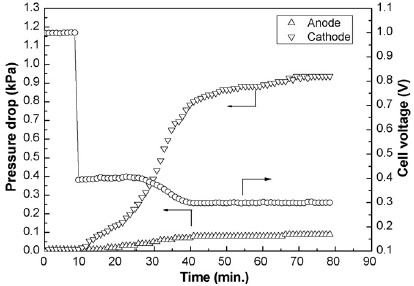
\includegraphics{Research_pictures/Fig1.jpg}
    \caption[short]{The change of cathode and anode voltage drop with time during flooding process}
\end{figure}
The detection methods based on electrochemical signals mainly include electrochemical impedance spectroscopy, current interruption method, and cyclic voltammetry, etc. Among them, electrochemical impedance spectroscopy is the most common hydration state detection method because it can distinguish different electrochemical processes and can be tested online \cite{yousfisteinerDiagnosisPolymerElectrolyte2011,chenOperationCharacteristicsCarbon2015}. The figure \ref{fig:figure1} shows the difference in fuel cell impedance spectra under different air humidity conditions. As the air humidity decreases, the value of the high-frequency impedance segment (i.e., the intercept of the impedance spectrum with the real axis) gradually increases, the impedance spectrum moves to the right, and the radius of the low-frequency arc segment also gradually increases \cite{hussainiVisualizationQuantificationCathode2009}, which can be used as an indicator of the hydration state of the fuel cell.
\par
When analyzing the relationship between impedance spectra and the internal hydration state of fuel cells, equivalent circuit models are often introduced. The model generally includes resistors, capacitors, inductors, and Warburg elements\cite{tangRecentProgressUse2020}. The model is capable of quantitatively analyzing the electrochemical process.  The key to this method is the establishment of equivalent models and parameter identification. Fouquet et al.[25] extended the standard capacitor to a constant phase element, proving that the three resistance values of the model are related to the relative humidity of the air supply. Zhang et al.[26] used a neural network method to complete parameter identification, and the predicted Nyquist plot almost completely coincides with the measured value, and by directly predicting the parameters of the equivalent circuit, they detailed the degree of influence of different processes on fuel cell performance. BMW proposed a method for online monitoring of impedance, which requires collecting five frequency points, divided into three groups to fit the Randles circuit, obtaining ohmic impedance, polarization resistance and double layer capacitance\cite{fouquetModelBasedPEM2006}. 
\par
However, the above methods are mostly suitable for single cells or low-power fuel cells. Applying them to high-power fuel cell doesn't gain any noticeable improvements\cite{tangRecentProgressUse2020,jiangMicrobialFuelCell2018,dotelliCombiningElectricalPressure2016,millerReviewPolymerElectrolyte2011,nagulapatiMachineLearningBased2023}, since the assembly structure, flow field structure, and operating conditions of high-power fuel cell stacks are significantly different from those of single cells and low-power stacks.  Therefore, the detection of the hydration state of high-power fuel cell systems is still in a relatively blank stage.
\par
Consequently, this study aims to investigate the hydration state of high-power fuel cell systems, construct, and validate a water balance model. Initially, the water balance model of the high-power fuel cell system is scrutinized, and a condensation-type exhaust water collection device is established to compute the water flow rate emanating from the fuel cell system. To authenticate the constructed water balance model, controlled variable experiments are executed under varying working temperatures, air metering ratios, and load currents. The experimental outcomes indicate that as the working temperature and air metering ratio escalate, the water flow rate emanating from the air side incrementally increases, and the water flow rate from the hydrogen side gradually diminishes. As the load current amplifies, the water flow rate emanating from both sides augments. Ultimately, predicated on the experimental data, the change rate of the internal water content of the fuel cell system under diverse conditions is calculated. The results reveal that under the same load current, as the working temperature and the air stoichiometric ratio augment, the change rate of the internal water content of the fuel cell system progressively decreases. Conversely, as the load current intensifies, the impact of the air stoichiometric ratio also incrementally escalates. Therefore, at low power, it is essential to maintain an appropriate working temperature, while at high power, upholding an appropriate metering ratio is of greater significance.
